\documentclass{IEEEtran}

\usepackage{cite}
\usepackage{amsmath,amssymb,amsfonts,esvect}
\usepackage{graphicx}
\usepackage{xcolor}
\usepackage{hyperref,url}
\usepackage{tikz}
\usetikzlibrary{decorations.pathreplacing}
\usepackage{float}

\newenvironment{Figure}
{\par\medskip\noindent\minipage{\linewidth}}
{\endminipage\par\medskip}

\DeclareMathOperator{\atantwo}{arctan2}

\begin{document}
% What happens when you lock a couple guys in a basement with nothing but
% 60 computers and a blackboard?
% They invent a new form of spacecraft guidance!
\title{Using Barometric Pressure Altitude to Verify and Improve GNSS/INS Surface Position Accuracy in Space Vehicle Ascent Guidance}

\author{%
	\IEEEauthorblockN{Spencer Bretz \hspace{1cm} Michael Turnbull}\\%
	\IEEEauthorblockA{%
        School of Electrical Engineering and Computer Science // Department of Physics\\%
		University of North Dakota\\%
		Grand Forks, ND 58203\\%
        \texttt{\{%
            \href{mailto:spencer.bretz@und.edu}{spencer.bretz},%
           \href{mailto:michael.turnbull@und.edu}{michael.turnbull}%
            \}@und.edu}%
    }
}

\date{\today}

\maketitle

\begin{abstract}
In this paper, we detail a method for determining a reduced set of Cartesian
coordinates relative to the Earth (or any planetary body with a sufficiently
studied atmosphere) given either barometrically-measured surface altitude or
ambient temperature, plus a known starting location, velocity, and flight time
for an ascending space vehicle.  While the accuracy of this method is not yet
known, it is worth further investigation to determine the feasibility and
efficiency of such a computation and whether or not it is beneficial to the
total accuracy of the vehicle's entire navigation system.
\end{abstract}

\begin{IEEEkeywords}
    barometer, GNSS, INS, space vehicle guidance, navigation error
\end{IEEEkeywords}

In any spacecraft ascent guidance system, a barometric pressure sensor
is vitally important for accurately computing the vehicle's altitude above
Earth's surface.  Tradition (and common sense) dictates that since a barometer
can only measure atmospheric pressure, the \emph{only} readings it can be used
for are pressure altitude and not location (latitude/longitude or Cartesian
coordinates).  However, it became apparent that since spacecraft
\href{https://xkcd.com/2087/}{don't always fly straight upwards}, there is a
difference in total distance traveled and barometric altitude.  This difference
is illustrated in figure \ref{fig:altdiff} by the equation
$\frac{\vec{Y}}{\lVert\vec{v}\rVert}t - \Delta y$.  Effectively, take the difference
between total distance traveled (represented by $\vec{v}t$) and the currently
measured barometric altitude ($\Delta y$) and compare them along the same
axis.

\begin{figure}[h]
\begin{centering}
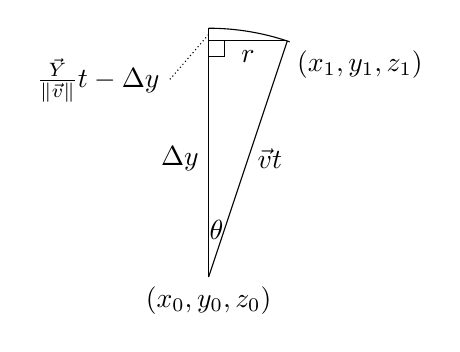
\begin{tikzpicture}
\draw (0,0) -- (0,3.16);
\draw (0,3) -- (1,3);
\draw (0,0) -- (1,3);
\draw (0,3.16) arc (90:71:3.16);

\draw (0.1,0.35) node[anchor=south] {$\theta$};
\draw (0, 1.5) node[anchor=east] {$\Delta y$};
\draw (0,0) node[anchor=north] {$(x_0, y_0, z_0)$};
\draw (0,2.8) -- (0.2,2.8) -- (0.2,3);
\draw (0.5,1.5) node[anchor=west] {$\vec{v}t$};
\draw (0.5,3) node[anchor=north] {$r$};
\draw (1,3) node[anchor=north west] {$(x_1, y_1, z_1)$};
\draw[densely dotted] (0,3.08) -- (-0.5,2.5);
\draw (-0.5,2.5) node[anchor=east] {$\frac{\vec{Y}}{\lVert\vec{v}\rVert}t - \Delta y$};
\end{tikzpicture}
\caption{Difference between distance traveled and barometric altitude}
\label{fig:altdiff}
\end{centering}
\end{figure}

Next, we account for error margins.  Assuming an angular size error $\alpha$
in the measurement of $\theta$ and an altimeter error margin $\beta$ defines an
ellipse lying in the $XY$ plane.  The equation for this ellipse is given
in equation \ref{eq:ellipse}.  It should be noted that this ellipse is not
aligned with the $X$ and $Y$ axis -- it is in fact rotated by an angle of
$-\theta$ as shown in figure \ref{fig:rotellipse}.  

This ellipse is defined by
either setting $E(x,y)$ (as defined in equation \ref{eq:ellipse}) equal to 1
or with parametric equations \ref{eq:para_el_x} and \ref{eq:para_el_y} in terms
of central angle $\phi$.  Note the semi-axes $s$ and $q$ are derived from the
error margins (not shown in any diagrams - $\alpha$ is the angular error in
$\theta$ and $\beta$ is the vertical error in $\Delta y$).

\begin{figure}[h]
\begin{centering}
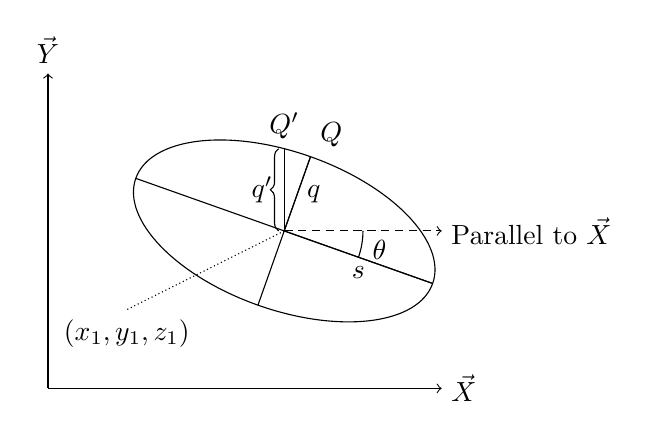
\begin{tikzpicture}
\draw[rotate=-19.5] (0,0) ellipse (2 and 1);
\draw[rotate=-19.5] (-2,0) -- (2,0);
\draw[rotate=-19.5] (0,-1) -- (0,1);
\draw[densely dotted] (0,0) -- (-2,-1);
\draw (-2,-1) node[anchor=north] {$(x_1,y_1,z_1)$};
\draw[rotate=-19.5] (0,0) -- (0,1) node[anchor=west,midway] {$q$};
\draw[rotate=-19.5] (0,0) -- (2,0) node[anchor=north,midway] {$s$};
\draw[->] (-3,-2) -- (2,-2);
\draw (2,-2) node[anchor=west] {$\vec{X}$};
\draw[->] (-3,-2) -- (-3,2);
\draw (-3,2) node[anchor=south] {$\vec{Y}$};

\draw (0,0) -- (0,1.044);
\draw[decorate,decoration={brace,amplitude=3pt},xshift=-2pt,yshift=0pt]
(0,0) -- (0,1.044) node[black,midway,yshift=0pt,xshift=-6pt] {$q'$};

\draw (0,1.044) node[anchor=south] {$Q'$};
\draw[rotate=-19.5] (0,1) node[anchor=south west] {$Q$};

\draw[densely dashed,->] (0,0) -- (2,0);
\draw (2,0) node[anchor=west] {Parallel to $\vec{X}$};
\draw (1,0) arc (0:-19.5:1);
\draw (1,0) node[anchor=north west] {$\theta$};
\end{tikzpicture}
\caption{Rotated ellipse in the $XY$ plane}
\label{fig:rotellipse}
\end{centering}
\end{figure}

Now that we have a valid set of points within error bounds (the set of points
contained within the ellipse, or where $E(x, y) \leq 1$), we can move into a
3D system.  Since we only know distance traveled and height, the actual
rocket location can be extrapolated to a ring around the $\vec{Y}$ axis.
Including the previously determined error ellipse, we can define a rotated
elliptical torus normal to the $\vec{Y}$ axis.  This rotation is shown in
figure \ref{fig:rotellipse}.

\begin{figure}{h}
\begin{centering}
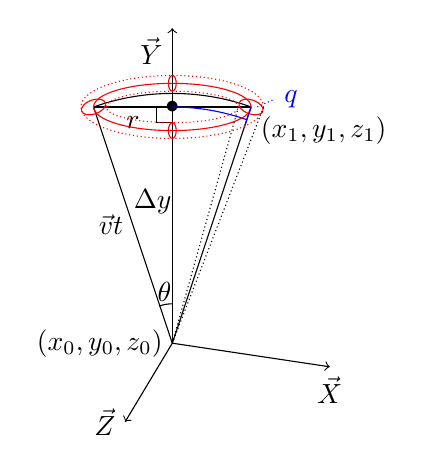
\begin{tikzpicture}
\draw[->] (0,0) -- (0,4);
\draw (-1,3) -- (1,3);
\draw (0,0) -- (1,3);
\draw (-1,3) arc (109.5:70.5:3);

\draw[->] (0,0) -- (2,-0.3);
\draw[->] (0,0) -- (-0.6,-1);

\draw (-0.25, 1.8) node {$\Delta y$};
\draw (0,4) node[anchor=north east] {$\vec{Y}$};
\draw (2,-0.3) node[anchor=north] {$\vec{X}$};
\draw (-0.6,-1) node[anchor=east] {$\vec{Z}$};
\draw (0,0) node[anchor=east] {$(x_0, y_0, z_0)$};
\draw (0,2.8) -- (-0.2,2.8) -- (-0.2,3);
\draw (-0.5,1.5) node[anchor=east] {$\vec{v}t$};
\draw (-0.5,3) node[anchor=north] {$r$};
\draw (0,3) node {$\bullet$};
\draw (1,3) node[anchor=north west] {$(x_1, y_1, z_1)$};
\draw (0,0) -- (-1,3);

\draw[blue] (0,3) arc (90:70.5:2.84);

\draw[red] (0,3) ellipse (1 and 0.3);
\draw[red,densely dotted] (0,3) ellipse (0.84 and 0.2);
\draw[red,densely dotted] (0,3) ellipse (1.16 and 0.4);

\draw[red,rotate around={-19.5:(1,3)}] (1,3) ellipse (0.16 and 0.09);
\draw[red,rotate around={19.5:(-1,3)}] (-1,3) ellipse (0.16 and 0.09);
\draw[red] (0,2.7) ellipse (0.05 and 0.1);
\draw[red] (0,3.3) ellipse (0.05 and 0.1);

\draw[densely dotted] (0,0) -- (0.84,3);
\draw[densely dotted] (0,0) -- (1.16,3);

\draw[blue] (1,3) -- (0.923,2.77);
\draw[blue,densely dotted] (1.08,3) -- (1.3,3.1);
\draw[blue] (1.3,3.1) node[anchor=west] {$q$};

\draw (0,0.5) arc (90:109.5:0.5);
\draw (-.1,0.65) node {$\theta$};
\end{tikzpicture}
\caption{Rotated elliptical torus about the $Y$ axis showing error margin in 3D}
\label{fig:errortorus}
\end{centering}
\end{figure}

At this point, we can begin the process of reducing error margins on estimations
from other navigation sources.  For each of the navigation sources (GNSS, INS,
INS postdiction, and any other forms in use), the same steps will be repeated.

First, we determine the angle in the $\vec{X}\vec{Z}$ plane that the point (which for
this loop we will call $P2 = (x_2, y_2, z_2)$ lies in and call this angle $\psi$.
The ultimate goal is to determine whether the point lies outside the torus,
and if it does, we can bring it to the edge of the torus.  Rather than rotate the
ellipse around the $\vec{Y}$ axis, which would be unnecessarily complex, we will
rotate the point $P2$ around the $\vec{Y}$ axis so that it lies in the $\vec{X}\vec{Y}$
plane.  We call this first transformed point $(x_{2a}, y_{2a}, z_{2a})$.  This is done
in equations \ref{eq:rotang_P2} and \ref{eq:p2rotate}.

Next, we need determine whether or not the point $(x_{2a}, y_{2a}, z_{2a})$ lies within
the ellipse previously defined.  Since the equation of a rotated ellipse is given in
equation \ref{eq:ellipse} and must be equal to 1 in order to form an ellipse, we can
simply check whether the function $E(x_{2a}, y_{2a})$ is less than or equal to 1.  If it
is, the point lies on or inside the ellipse; and if not, the point lies outside.

Now that we know where the point is, we can determine what action must be taken.  This
is again fairly simple -- if the point lies outside the ellipse, we transform it to the
boundary of the ellipse.  To actually perform this transformation, we first determine the
interior angle of the point $\gamma$ given in equation \ref{eq:gamma}.  Then, we take
the appropriate action (scale it to the ellipse) in equation \ref{eq:scaletoellipse}, and
finally rotate it back around the $\vec{Y}$ axis to match the original angle in equation
\ref{eq:P2backaround}.

Now, the point $(x_{2c}, y_{2c}, z_{2c})$ has been reduced if possible.  The steps can now
be repeated with another point from another navigation source to further reduce error.

\begin{figure*}[h]
\begin{centering}
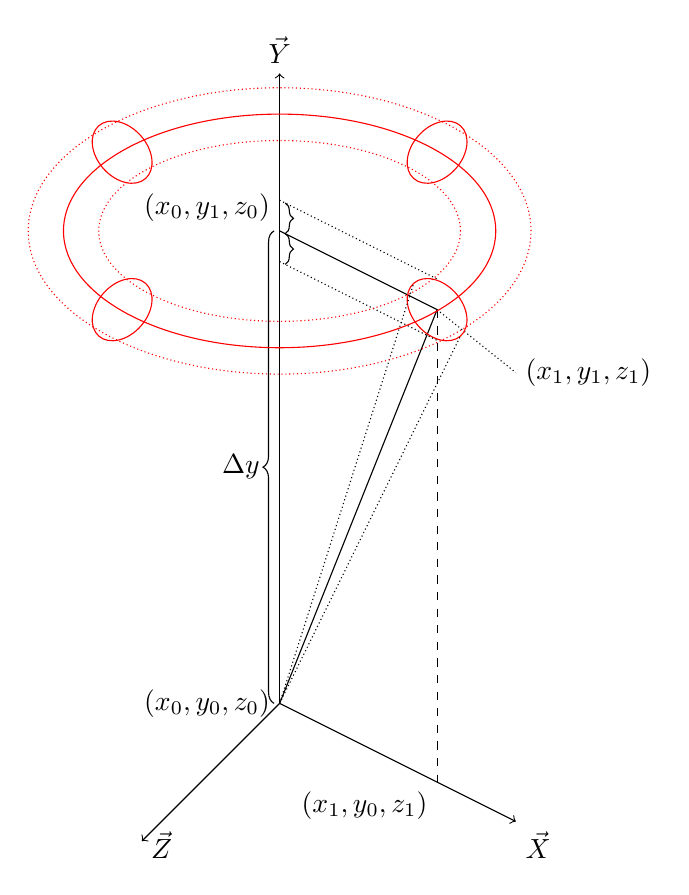
\begin{tikzpicture}
% Axes
\draw[->] (0,0) -- (0,8);          \draw (0,8) node[anchor=south] {$\vec{Y}$};
\draw[->] (0,0) -- (-1.75,-1.75);  \draw (-1.5,-1.5) node[anchor=north] {$\vec{Z}$};
\draw[->] (0,0) -- (3,-1.5);       \draw (3,-1.5) node[anchor=north west] {$\vec{X}$};

% X-plane offset:  26.57
% Theta offset:    21.80
% X+theta offsets: 48.37

% Spacecraft points
\draw (0,6) -- (2,5);
\draw (3,4.2) node[anchor=west] {$(x_1, y_1, z_1)$};
\draw[densely dotted] (2,5) -- (3,4.2);
\draw[dashed] (2,5) -- (2,-1); 
\draw (0,0) -- (2,5);
\draw (0,0) node[anchor=east] {$(x_0, y_0, z_0)$};
\draw (2,-1) node[anchor=north east] {$(x_1, y_0, z_1)$};
\draw (0,6) node[anchor=south east] {$(x_0, y_1, z_0)$};

% Errors in theta & deltaY -- alpha & beta
\draw[red,rotate around={-48.37:(2,5)}] (2,5) ellipse (0.4478 and 0.316);
\draw[densely dotted] (0,0) -- (2.297,4.665);    % alpha below
\draw[densely dotted] (0,0) -- (1.703,5.335);    % alpha above
\draw[densely dotted] (0,6.3896) -- (2,5.3896);  % beta above
\draw[densely dotted] (0,5.6103) -- (2,4.6103);  % beta below
\draw[decorate,decoration={brace,amplitude=4pt},xshift=-2pt,yshift=0pt]
  (0,0) -- (0,6) node[black,midway,yshift=0pt,xshift=-12pt] {$\Delta y$};
\draw[decorate,decoration={brace,amplitude=3pt},xshift=2pt,yshift=-1pt]
  (0,6.3896) -- (0,6);
\draw[decorate,decoration={brace,amplitude=3pt},xshift=2pt,yshift=-1pt]
  (0,6) -- (0,5.6103);

% Torus time!
\draw[red,densely dotted] (0,6) ellipse (2.297 and 1.1485);    % inner boundary
\draw[red,densely dotted] (0,6) ellipse (3.1926 and 1.8185);   % outer boundary
\draw[red] (0,6) ellipse (2.7448 and 1.4835);                  % central ring
\draw[red,rotate around={48.37:(-2,5)}] (-2,5) ellipse (0.4478 and 0.316);
\draw[red,rotate around={-48.37:((-2,7)}] (-2,7) ellipse (0.4478 and 0.316);
\draw[red,rotate around={48.37:(2,7)}] (2,7) ellipse (0.4478 and 0.316);

\end{tikzpicture}
\caption{Blown-up figure depicting all aspects of the problem}
\label{fig:big}
\end{centering}
\end{figure*}

\begin{figure*}[h]
\begin{subequations}
\begin{equation}
s = \lVert\vec{v}\rVert t\tan(\alpha)
\label{eq:s}
\end{equation}
\begin{equation}
q' = \beta
\label{eq:qprime}
\end{equation}
\begin{equation}
q = \csc(\theta)\left(-\left(x_1+s\cos(\theta)\right)\right), \textrm{if} \sin(\theta) \neq 0
\end{equation}
\begin{equation}
E(x,y) = \frac{\left((x-x_1)\cos(\theta) + (y-y_1)\sin(\theta)\right)^2}{s^2} + \frac{\left((x-x_1)\cos(\theta) - (y-y_a)\sin(\theta)\right)^2}{q^2}
\label{eq:ellipse}
\end{equation}
\begin{equation}
E_x(\phi) = s\cos(\phi)\cos(-\theta) - q\sin(\phi)\sin(-\theta) + x_1
\label{eq:para_el_x}
\end{equation}
\begin{equation}
E_y(\phi) = s\cos(\phi)\sin(-\theta) + q\sin(\phi)\cos(-\theta) + y_1
\label{eq:para_el_y}
\end{equation}
\end{subequations}
\begin{subequations}
\begin{equation}
\psi = \atantwo(z_2,x_2)
\label{eq:rotang_P2}
\end{equation}
\begin{equation}
(x_{2a}, y_{2a}, z_{2a}) = (z_2\sin(-\psi)+x_2\cos(-\psi), y_2, z_2\cos(-\psi)-x_2\sin(-\psi))
\label{eq:p2rotate}
\end{equation}
\end{subequations}
\begin{subequations}
\begin{equation}
\gamma = \atantwo(y_{2a} - y_1, x_{2a} - x_1)
\label{eq:gamma}
\end{equation}
\begin{equation}
(x_{2b}, y_{2b}, z_{2b}) =
\begin{cases}
    (x_{2a}, y_{2a}, z_{2a}) & E(x_{2a}, y_{2a}) \leq 1 \\
    (E_x(\gamma), E_y(\gamma), z_{2a}) & E(x_{2a}, y_{2a}) > 1
\end{cases}
\label{eq:scaletoellipse}
\end{equation}
\begin{equation}
(x_{2c}, y_{2c}, z_{2c}) = (z_{2b}\sin(\psi) + x_{2b}\cos(\psi),y_{2b},
z_{2b}\cos(\psi)-x_{2b}\sin(\psi))
\label{eq:P2backaround}
\end{equation}
\end{subequations}
\end{figure*}

\end{document}
